\chapter{Xây dựng phiên bản thử nghiệm}
\section{Công nghệ sử dụng}
Để hiện thực hệ thống, nhóm quyết định sử dụng các công nghệ sau:
\begin{itemize}
    \item ReactJS: Hiện thực UI, frontend.
    \item Java Springboot: Hiện thực microservice, backend.
    \item PostgresSQL: Hệ cơ sở dữ liệu lưu trữ thông tin.
    \item Kubernetes: Deploy các microservice.
    \item Minikube: Chạy Kubernetes cluster trên local.
    \item Terraform: Khởi tạo 
\end{itemize}

\section{Giới hạn phạm vi}
\subsection{Về mặt nghiệp vụ}
\noindent Sau khi bàn bạc, nhóm đi tới thống nhất là sẽ hiện thực phần Trang chủ (Home page - Catalog), vì đó là thành phần mà người dùng sẽ gặp đầu tiên khi bắt đầu truy cập vào hệ thống.
\subsection{Về mặt thành phần hệ thống}
\noindent Sau khi cân nhắc kỹ lưỡng, để đảm bảo cho phiên bản demo thể hiện được trọn vẹn và đầy đủ nhất các tính chất cốt lõi của hệ thống, nhóm đã giới hạn phạm vi hiện thực của hệ thống xuống còn các thành phần như sau:
\begin{itemize}
    \item Frontend: Trang chủ - Catalog, thể hiện danh sách các mặt hàng đang được bày bán 
    \item Backend: Catalog service, cung cấp API danh sách sản phẩm.
    \item Minikube cluster: Cung cấp môi trường Kubernetes cluster local trên máy tính cá nhân.
    \item Deployment: Thành phần cơ bản nhất của hệ thống, dùng để quản lý trực tiếp các pod.
    \item Service: Một lớp ảo hóa để các thành phần khác có thể truy cập tới các pod.
    \item Ingress: Đóng vai trò như reverse proxy, cung cấp API gateway để kết nối từ bên ngoài cluster tới service.
    \item Horizontal Pod Autoscaler: Dùng để tăng hoặc giảm số pod một cách tự động, dựa trên các thông số (metrics) của chính các pod đó.
\end{itemize}
\section{Nội dung hiện thực}
\subsection{Hiện thực frontend và backend}
\noindent Sau khi có một ứng dụng hoàn chỉnh, có thể hiển thị được thông tin mặt hàng, ta đóng gói nó thành Docker image và đẩy lên Docker Hub.\\[0.5cm]
Dockerfile của frontend có nội dung như sau:
\begin{lstlisting}[language=docker]
# Use an official Node runtime as a parent image
FROM node:18 AS builder

# Set the working directory in the container
WORKDIR /app

# Copy package.json and package-lock.json to the container
COPY package.json ./

# Install dependencies
RUN npm install

# Copy the rest of the application code to the container
COPY . .

# Build the Vite React application
RUN npm run build

# Use an official Nginx runtime as a parent image
FROM nginx:alpine

# Copy the build output from the builder stage to the nginx web root
COPY --from=builder /app/dist /usr/share/nginx/html

# Expose port 80
EXPOSE 80
\end{lstlisting}

Dockerfile của backend có nội dung như sau:

\begin{lstlisting}[language=docker]
# Use an official OpenJDK runtime as a base image with Java 17
FROM eclipse-temurin:17-jdk-alpine

# Set the working directory to /app
WORKDIR /app

# Copy the current directory contents into the container at /app
COPY . /app

# Build the Spring Boot application
RUN ./mvnw package -DskipTests

# Expose the port that your Spring Boot application will run on
EXPOSE 80

# Define the command to run your application
CMD ["java", "-jar", "target/catalog-0.0.1-SNAPSHOT.jar"]
\end{lstlisting}

\subsection{Hiện thực Deployment và Service}
\noindent Ta sử dụng terraform để khởi tạo các service trên, tương ứng với mỗi microservice frontend và backend.
\subsubsection{Với frontend}
\noindent Với frontend, khi được đưa lên production, service sẽ được build thành định dạng html, css truyền thống, đi kèm với file javascript chứa logic, và được cung cấp bởi Nginx server, do đó mặc định port sẽ là 80 (HTTP).
\begin{lstlisting}[language=terraform]
resource "kubernetes_deployment" "catalog-fe-deploy" {
  metadata {
    name = "catalog-fe-deploy"
    labels = { app = "catalog-fe", tier = "frontend" }
  }
  spec {
    replicas = 1
    selector {
      match_labels = { app = "catalog-fe-pod", tier = "frontend" }
    }
    template {
      metadata {
        name = "catalog-fe-pod"
        labels = { app = "catalog-fe-pod", tier = "frontend"}
      }
      spec {
        container {
          name = "catalog-fe"
          image = "hoanganhleboy/catalog-fe:latest"
          port { container_port = 80 }
          env {
            name = "CONTENT"
            value = "This is the string from k8s"
          }
          image_pull_policy = "Always"
        }
      }
    }
  }
}

resource "kubernetes_service" "catalog-fe-service" {
  metadata {
    name = "catalog-fe-service"
    labels = { app = "catalog-fe-service", tier = "frontend" }
  }
  spec {
    selector = { app = "catalog-fe-pod", tier = "frontend"}
    port {
      protocol = "TCP"
      port = 80
      target_port = 80
    }
    type = "NodePort"
  }
}
\end{lstlisting} 
\subsubsection{Với backend}
\noindent Catalog microservice sau khi được build thành image sẽ được chạy từ file .jar, thông qua JVM.
\begin{lstlisting}[language=terraform]
resource "kubernetes_deployment" "catalog-ms-deploy" {
  metadata {
    name = "catalog-ms-deploy"
    labels = { app = "catalog-ms", tier = "backend" }
  }
  spec {
    replicas = 1
    selector {
      match_labels = { app = "catalog-ms-pod", tier = "backend" }
    }
    template {
      metadata {
        name = "catalog-ms-pod"
        labels = { app = "catalog-ms-pod", tier = "backend"}
      }
      spec {
        container {
          name = "catalog-ms"
          image = "hoanganhleboy/catalog-ms"
          port { container_port = 8090 } // This port the same with port in the code.
          resources {
            requests = {
              cpu = "256m"
              memory = "128Mi"
            }
            limits = {
              cpu = "256m"
              memory = "128Mi"
            }
          }
        }
      }
    }
  }
}

resource "kubernetes_service" "catalog-ms-service" {
  metadata {
    name = "catalog-ms-service"
    labels = { app = "catalog-ms-service", tier = "backend" }
  }
  spec {
    selector = { app = "catalog-ms-pod", tier = "backend"}
    port {
      protocol = "TCP"
      port = 8090 // port expose to outside
      target_port = 80 // This port the same with port in the code.
    }
    type = "NodePort"
  }
}
\end{lstlisting}
\subsection{Hiện thực Ingress}
\noindent Ingress hiện tại đóng vai trò là reverse proxy, expose các Kubernetes service ra bên ngoài cluster.
\begin{lstlisting}[language=yaml]
apiVersion: networking.k8s.io/v1
kind: Ingress
metadata:
  name: example-ingress
  annotations:
    nginx.ingress.kubernetes.io/enable-directory-listing: "true"
    nginx.ingress.kubernetes.io/rewrite-target: /$2
spec:
  rules:
    - http:
        paths:
          - pathType: Prefix
            path: /backend(/|$)(.*)
            backend:
              service:
                name: catalog-ms-service
                port:
                  number: 80
          - pathType: Prefix
            path: /frontend/?(.*)
            # path: /
            backend:
              service:
                name: catalog-fe-service
                port:
                  number: 80
---

\end{lstlisting}
\subsection{Hiện thực Horizontal Pod Autoscaler}
\noindent Horizontal Pod Autoscaler (HPA) được sử dụng để giúp deployment có thể scale lên và scale xuống số lượng pod tùy theo thông số nào đó của hệ thống. HPA được hiện thực như sau:
\begin{lstlisting}[language=yaml]
apiVersion: autoscaling/v2
kind: HorizontalPodAutoscaler
metadata:
  name: catalog-ms-hpa
spec:
  maxReplicas: 10
  metrics:
  - resource:
      name: cpu
      target:
        averageUtilization: 10
        type: Utilization
    type: Resource
  minReplicas: 1
  scaleTargetRef:
    apiVersion: apps/v1
    kind: Deployment
    name: catalog-ms-deploy
  behavior:
    scaleUp:
      selectPolicy: Max
      stabilizationWindowSeconds: 60
      policies:
      # number of pods that scale in a period of time
        - periodSeconds: 30
          type: Pods
          value: 4
    scaleDown:
      selectPolicy: Min
      stabilizationWindowSeconds: 60
      policies:
      # number of pods that scale in a period of time
        - periodSeconds: 30
          type: Pods
          value: 4
\end{lstlisting}
\section{Kiểm thử hệ thống}
\subsection{Thiết lập}
\noindent Sử dụng minikube, ta tạo một cluster với driver là docker (chạy trên nền docker), bằng câu lệnh \lstinline|minikube start --driver=docker|. Sau đó, ta cần kích hoạt 2 add on cần thiết cho ingress và HPA bằng 2 câu lệnh sau:
\begin{itemize}
  \item \lstinline|minikube addons enable ingress|
  \item \lstinline|minikube addons enable metrics-server|
\end{itemize}
Với addon ingress, ta có thể thiết lập và cấu hình ingress cho cluster. Addon metrics-server đóng vai trò cung cấp, theo dõi các thông số của pod (cpu, memory) nhằm phục vụ cho HPA.\\[0.5cm]
Sau đó, ta sẽ chạy cặp lệnh \lstinline|terraform init| để terraform tải và thiết lập sẵn các dependency cần thiết, và \lstinline|terraform apply --auto-approve| để khởi tạo các dịch vụ Kubernetes được viết bằng terraform.\\[0.5cm]
Với các dịch vụ được viết bằng yaml, ta cần chạy lệnh \lstinline|kubectl apply -f <file_name>| với \lstinline|<file_name>| là tên file config được viết bằng yaml.
\subsection{Kiểm tra tính sẵn sàng - availability}
\noindent Để kiếm tra tính sẵn sàng của hệ thống, ta sẽ thử xóa pod đi xem chuyện gì sẽ xảy ra.\\[0.5cm]
Đây là trạng thái ban đầu của các pod:
\begin{figure}[H]
  \begin{center}
  \includegraphics[scale=0.45]{images/hanh/pod_before_delete.png}
  \caption{Hình ảnh trước khi xóa pod}
  \end{center}
\end{figure}
Còn đây là hình ảnh sau khi vừa xóa:
\begin{figure}[H]
  \begin{center}
  \includegraphics[scale=0.45]{images/hanh/pod_after_delete.png}
  \caption{Hình ảnh sau khi vừa xóa pod}
  \end{center}
\end{figure}
Như ta nhìn thấy trong hình 5.1 và 5.2, khi một pod vừa bị xóa, ngay lập tức một pod khác được khởi động ngay lập tức, thế chỗ cho pod vừa bị xóa. Như vậy, ta có thể kết luận rằng, khi triển khai hệ thống bằng Kubernetes, cụ thể là Deployment, tính sẵn sàng - availability của hệ thống được đảm bảo.
\subsection{Kiếm tra tính mở rộng - scalability}
\subsubsection{Manual scaling}
\noindent Tính mở rộng là việc hệ thống có thể tạo ra thêm nhiều bản sao của microservice, chạy song song với nhau nhằm đáp ứng được lượng request trên giây tương ứng của người dùng. Với Kubernetes, ta có thể dễ dàng scale up hay scale down hệ thống bằng tay thông qua việc điều chỉnh miền \lstinline|replicas| trong file config của Deployment.\\[0.5cm]
Ví dụ như hình 5.3 dưới đây, khi ta tăng số lượng pod của catalog-ms từ 1 lên 3
\begin{figure}[H]
  \begin{center}
    \includegraphics[scale=0.45]{images/hanh/catalog_ms_scale_up.png}
    \caption{Hình ảnh khi scale số pod từ 1 lên 3}
  \end{center}
\end{figure}
Ngay lập tức đã có thêm 2 pod mới được tạo ra như hình. Sau đó, khi ta giảm xuống 1 lại thì:
\begin{figure}[H]
  \begin{center}
    \includegraphics[scale=0.45]{images/hanh/catalog_ms_scale_down.png}
    \caption{Hình ảnh khi scale số pod từ 3 xuống 1}
  \end{center}
\end{figure}
Như hình 5.4, ta thấy ngay lập tức có 2 pod bị xóa đi để đảm bảo số lượng pod trong cluster về đúng số lượng quy định.

\subsubsection{Auto scaling}
Tuy nhiên, trên thực tế, việc scale thủ công như trên sẽ gây tiêu tốn tài nguyên về cả nhân lực và vật lực kha khá, do cần phải có sự can thiệp trực tiếp của con người, và cũng cần con người giám sát 24/24 để đảm bảo có thể điều chỉnh lượng pod phù hợp với nhu cầu lúc đó. Do đó, tốt hơn hết là ta nên thiết lập để Kubernetes có thể thực hiện việc đó một cách tự động thay cho chúng ta, và đó là khi ta cần dùng tới HPA - Horizontal Pod Autoscaler.\\[0.5cm]
Bài kiểm tra bao gồm các bước sau:
\begin{enumerate}
  \item Triển khai Deployment, Service, và HPA cho đối tượng muốn kiểm tra, ở đây là Catalog backend microservice.
  \item Khởi tạo một pod có chứa container được chạy từ image busybox, pod này sẽ cung cấp cho chúng ta môi trường linux shell. Ta sau đó viết 1 đoạn script tạo một vòng lặp vô hạn gọi tới API của Catalog backend microservice.
  \item Sử dụng câu lệnh \lstinline|kubectl get hpa --watch| để theo dõi trạng thái của HPA. Một thời gian sau, khi lượng pod đã được scale tới tối đa, ta tắt script để ngưng gọi API. 
  \item Lại đợi một khoảng thời gian, số pod đã được scale về mức tối thiểu. 
\end{enumerate}
\begin{figure}[H]
  \begin{center}
    \includegraphics[scale=0.19]{images/hanh/HPA_CPU_scale.png}
    \caption{Kết quả cuộc thử nghiệm}
  \end{center}
\end{figure}
\noindent \textbf{Mô tả thí nghiệm:} Trong hình 5.5, ta có thể thấy khi bắt đầu gọi API liên tục tới Catalog backend server, thì CPU load bắt đầu tăng mạnh. Khi CPU load vượt ngưỡng 10\% thì HPA sẽ được kích hoạt để tăng số pod trong deployment lên, nhằm mục đích làm giảm PCU load xuống. Tuy nhiên, một thời gian ngắn sau vì CPU load tiếp tục vượt ngưỡng nên HPA lại tiếp tục được kích hoạt tiếp để tăng thêm số pod ở deployment. Việc này chỉ dừng lại cho đến khi số pod đã đạt ngưỡng tối đa cho phép, hoặc CPU load ổn định không tiếp tục vượt ngưỡng nữa thì thôi.\\[0.5cm]
Sau khi đã scale số pod lên đến mức tối đa là 10, ta terminate busybox đi để ngừng việc gửi request tới Catalog microservice. Lúc này CPU load giảm mạnh xuống còn 0\%. Sau một khoảng thời gian, HPA lại được kích hoạt để giảm số pod xuống. Khi giảm pod, nhận thấy CPU load vẫn tiếp tục dưới ngưỡng, HPA tiếp tục được kích hoạt để giảm tiếp số pod xuống, đến khi nào CPU load xấp xỉ với ngưỡng, hoặc khi đạt đến số pod tối thiểu, ở đây là 1 pod.

\section{Xây dựng tính năng autoscaling với custom metrics (các thông số tùy chỉnh)}
% Tham khảo chính từ 2 bài viết: https://dev.to/k6/how-to-autoscale-kubernetes-pods-with-keda-testing-with-k6-4nl9\influx-grafana và https://devopscube.com/setup-prometheus-monitoring-on-kubernetes/

\subsection{Định nghĩa}
\noindent Theo Google Cloud Platform\footnote{Dựa theo link: https://cloud.google.com/kubernetes-engine/docs/concepts/custom-and-external-metrics}, một \textit{custom metric} sẽ được truyền từ ứng dụng của bạn mà đang chạy trên Kubernetes.
\subsection{Đặt vấn đề}
\noindent Việc scale theo CPU và memory không hiệu quả với rest api.
\subsection{Cơ sở lý thuyết}
\noindent Nói về việc prometheus dùng để thu thâp và cung cấp api server cho external metrics. Keda cung cấp ScaledObject, được build dựa trên HPA để phục vụ cho việc scale dựa trên các metric thu thập từ prometheus.\\
\noindent Có thể để các tóm tắt bài viết vào đây.
\subsection{Các công nghệ được sử dụng}
\subsubsection{Prometheus}
% TODO: Các phần này cần tự tìm thêm các nguồn khác để tìm hiểu
\subsubsection{Keda}
% TODO: Các phần này cần tự tìm thêm các nguồn khác để tìm hiểu
\subsubsection{k6}
% TODO: Các phần này cần tự tìm thêm các nguồn khác để tìm hiểu

\subsection{Các bước thực hiện}
\noindent Để có thể scale một service theo request, ta cần hiện thực các dịch vụ sau vào cluster:
\begin{itemize}
  \item Prometheus server
  \item Keda runtime.
\end{itemize}
Các bước thực hiện cụ thể sẽ được mô tả ở các tiểu mục bên dưới.
\subsubsection{Hiện thực prometheus server}
\noindent Để hiện thực Prometheus server, ta cần làm theo các bước sau:\footnote{https://devopscube.com/setup-prometheus-monitoring-on-kubernetes/}
% \begin{enumerate}[label=\textbf{Bước \arabic*:}, leftmargin=*]
\begin{itemize}
  \item \textbf{Bước 1: Tạo Namespace và ClusterRole.}\\[0.2cm]
  Ta sẽ tạo một namespace riêng cho Prometheus server và các service đi theo nó, mục đích là để tách biệt chúng ra khỏi các service phục vụ cho các yêu cầu khác của hệ thống.\\[0.2cm]
  Ta tạo namespace \textbf{monitoring} bằng câu lệnh \lstinline|kubectl create namespace monitoring|.\\[0.2cm]
  Sau đó, ta áp dụng config Cluster Role dưới đây vào cluster:
  \begin{lstlisting}[language=yaml]
apiVersion: rbac.authorization.k8s.io/v1
kind: ClusterRole
metadata:
  name: prometheus
rules:
- apiGroups: [""]
  resources:
  - nodes
  - nodes/proxy
  - services
  - endpoints
  - pods
  verbs: ["get", "list", "watch"]
- apiGroups:
  - extensions
  resources:
  - ingresses
  verbs: ["get", "list", "watch"]
- nonResourceURLs: ["/metrics"]
  verbs: ["get"]
---
apiVersion: rbac.authorization.k8s.io/v1
kind: ClusterRoleBinding
metadata:
  name: prometheus
roleRef:
  apiGroup: rbac.authorization.k8s.io
  kind: ClusterRole
  name: prometheus
subjects:
- kind: ServiceAccount
  name: default
  namespace: monitoring

  \end{lstlisting}
  \item \textbf{Bước 2: Tạo Config map để mở rộng cấu hình của Prometheus}\\[0.2cm]
  Prometheus, theo như ở phần trên, có thể đóng rất nhiều vai trò khác nhau trong một hệ thống. Do đó, việc cần điểu chỉnh cấu hình của nó là điều thường xuyên xảy ra. Thay vì cần phải build lại image của Prometheus mỗi khi cấu hình được điều chỉnh, thì nay ta có thể đem những cấu hình đó ra ngoài dưới dạng 1 file config map, từ đó tiết kiệm thời gian áp dụng thay đổi, thay vì phải build lại image, rồi push image lên hub, cuối cùng là kéo về cluster, thì ta chỉ cần khởi đọng lại prometheus pod là được.\\[0.2cm]
  Cấu hình Config map của prometheus như sau:
  \begin{lstlisting}[language=yaml]
apiVersion: v1
kind: ConfigMap
metadata:
  name: prometheus-server-conf
  labels:
    name: prometheus-server-conf
  namespace: monitoring
data:
  prometheus.rules: |-
    groups:
    - name: devopscube demo alert
      rules:
      - alert: High Pod Memory
        expr: sum(container_memory_usage_bytes) > 1
        for: 1m
        labels:
          severity: slack
        annotations:
          summary: High Memory Usage
  prometheus.yml: |-
    global:
      scrape_interval: 5s
      evaluation_interval: 5s
    rule_files:
      - /etc/prometheus/prometheus.rules
    alerting:
      alertmanagers:
      - scheme: http
        static_configs:
        - targets:
          - "alertmanager.monitoring.svc:9093"
    scrape_configs:
      - job_name: 'node-exporter'
        kubernetes_sd_configs:
          - role: endpoints
        relabel_configs:
        - source_labels: [__meta_kubernetes_endpoints_name]
          regex: 'node-exporter'
          action: keep
      - job_name: 'kubernetes-apiservers'
        kubernetes_sd_configs:
        - role: endpoints
        scheme: https
        tls_config:
          ca_file: /var/run/secrets/kubernetes.io/serviceaccount/ca.crt
        bearer_token_file: /var/run/secrets/kubernetes.io/serviceaccount/token
        relabel_configs:
        - source_labels: [__meta_kubernetes_namespace, __meta_kubernetes_service_name, __meta_kubernetes_endpoint_port_name]
          action: keep
          regex: default;kubernetes;https
      - job_name: 'kubernetes-nodes'
        scheme: https
        tls_config:
          ca_file: /var/run/secrets/kubernetes.io/serviceaccount/ca.crt
        bearer_token_file: /var/run/secrets/kubernetes.io/serviceaccount/token
        kubernetes_sd_configs:
        - role: node
        relabel_configs:
        - action: labelmap
          regex: __meta_kubernetes_node_label_(.+)
        - target_label: __address__
          replacement: kubernetes.default.svc:443
        - source_labels: [__meta_kubernetes_node_name]
          regex: (.+)
          target_label: __metrics_path__
          replacement: /api/v1/nodes/${1}/proxy/metrics
      - job_name: 'kubernetes-pods'
        kubernetes_sd_configs:
        - role: pod
        relabel_configs:
        - source_labels: [__meta_kubernetes_pod_annotation_prometheus_io_scrape]
          action: keep
          regex: true
        - source_labels: [__meta_kubernetes_pod_annotation_prometheus_io_path]
          action: replace
          target_label: __metrics_path__
          regex: (.+)
        - source_labels: [__address__, __meta_kubernetes_pod_annotation_prometheus_io_port]
          action: replace
          regex: ([^:]+)(?::\d+)?;(\d+)
          replacement: $1:$2
          target_label: __address__
        - action: labelmap
          regex: __meta_kubernetes_pod_label_(.+)
        - source_labels: [__meta_kubernetes_namespace]
          action: replace
          target_label: kubernetes_namespace
        - source_labels: [__meta_kubernetes_pod_name]
          action: replace
          target_label: kubernetes_pod_name
      - job_name: 'kube-state-metrics'
        static_configs:
          - targets: ['kube-state-metrics.kube-system.svc.cluster.local:8080']
      - job_name: 'kubernetes-cadvisor'
        scheme: https
        tls_config:
          ca_file: /var/run/secrets/kubernetes.io/serviceaccount/ca.crt
        bearer_token_file: /var/run/secrets/kubernetes.io/serviceaccount/token
        kubernetes_sd_configs:
        - role: node
        relabel_configs:
        - action: labelmap
          regex: __meta_kubernetes_node_label_(.+)
        - target_label: __address__
          replacement: kubernetes.default.svc:443
        - source_labels: [__meta_kubernetes_node_name]
          regex: (.+)
          target_label: __metrics_path__
          replacement: /api/v1/nodes/${1}/proxy/metrics/cadvisor
      - job_name: 'kubernetes-service-endpoints'
        kubernetes_sd_configs:
        - role: endpoints
        relabel_configs:
        - source_labels: [__meta_kubernetes_service_annotation_prometheus_io_scrape]
          action: keep
          regex: true
        - source_labels: [__meta_kubernetes_service_annotation_prometheus_io_scheme]
          action: replace
          target_label: __scheme__
          regex: (https?)
        - source_labels: [__meta_kubernetes_service_annotation_prometheus_io_path]
          action: replace
          target_label: __metrics_path__
          regex: (.+)
        - source_labels: [__address__, __meta_kubernetes_service_annotation_prometheus_io_port]
          action: replace
          target_label: __address__
          regex: ([^:]+)(?::\d+)?;(\d+)
          replacement: $1:$2
        - action: labelmap
          regex: __meta_kubernetes_service_label_(.+)
        - source_labels: [__meta_kubernetes_namespace]
          action: replace
          target_label: kubernetes_namespace
        - source_labels: [__meta_kubernetes_service_name]
          action: replace
          target_label: kubernetes_name
  \end{lstlisting}
  \item \textbf{Bước 3: Tạo một Prometheus Deployment}\\[0.2cm]
  Sau khi chuẩn bị sẵn sàng các dịch vụ hỗ trợ đi kèm, ta có thể khởi tạo một deployment cho Prometheus server theo config dưới đây.
  \begin{lstlisting}[language=yaml]
apiVersion: apps/v1
kind: Deployment
metadata:
  name: prometheus-deployment
  namespace: monitoring
  labels:
    app: prometheus-server
spec:
  replicas: 1
  selector:
    matchLabels:
      app: prometheus-server
  template:
    metadata:
      labels:
        app: prometheus-server
    spec:
      containers:
        - name: prometheus
          image: prom/prometheus
          args:
            - "--config.file=/etc/prometheus/prometheus.yml"
            - "--storage.tsdb.path=/prometheus/"
          ports:
            - containerPort: 9090
          volumeMounts:
            - name: prometheus-config-volume
              mountPath: /etc/prometheus/
            - name: prometheus-storage-volume
              mountPath: /prometheus/
      volumes:
        - name: prometheus-config-volume
          configMap:
            defaultMode: 420
            name: prometheus-server-conf
  
        - name: prometheus-storage-volume
          emptyDir: {}
  \end{lstlisting}
  Khởi tạo thành công, ta có thể nhìn thấy sự xuất hiện của Prometheus pod và deployment ở namespace \textbf{monitoring} như hình dưới.
  \begin{figure}[H]
    \begin{center}
      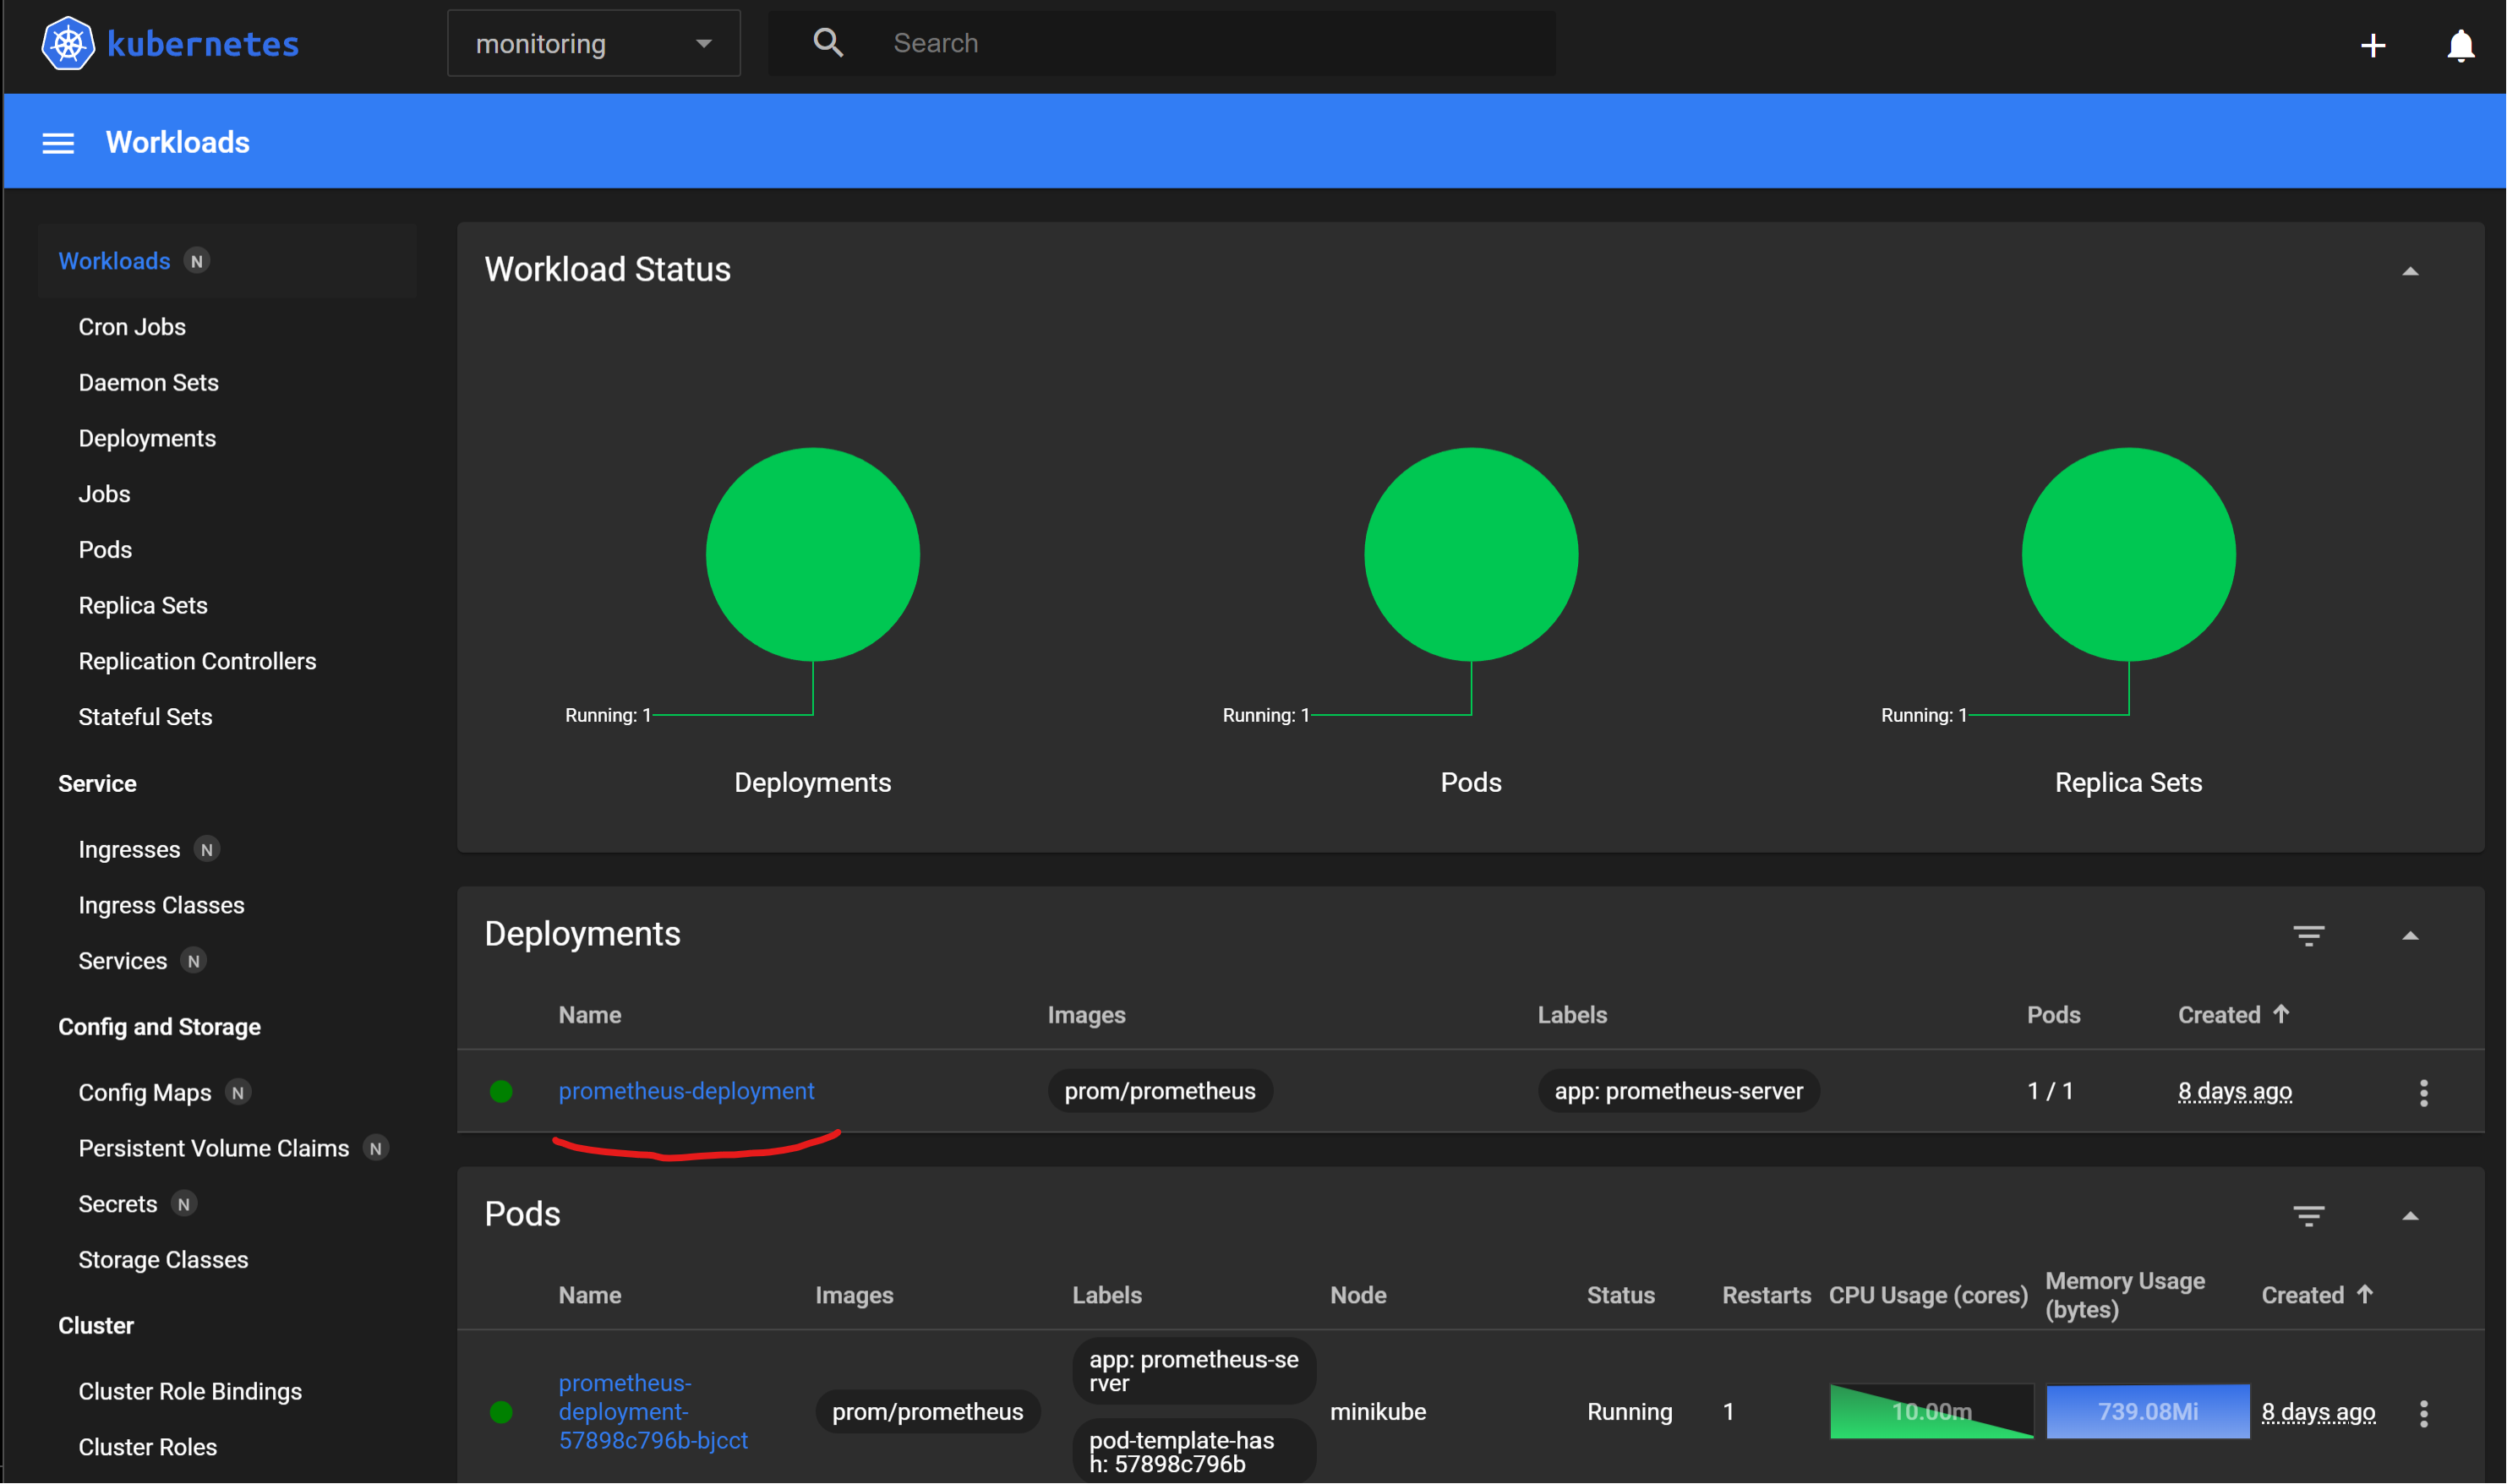
\includegraphics[scale = 0.4]{images/hanh/prometheus-deployment.png}
      \caption{Prometheus pod và deployment được thể hiện ở minikube cluster dashboard}
    \end{center}
    \label{}
  \end{figure}
  \item \textbf{Bước 4: Kết nối tới Prometheus Dashboard}\\[0.2cm]
  Sau khi đã cài đặt đầy đủ Prometheus server và các dịch vụ đi kèm, ta có thể truy cập vào dashboard của Prometheus để xem các thông số. Ví dụ với minikube cluster, ta có thể dùng lệnh \lstinline|minikube service prometheus-service| để mở cổng truy cập, cho phép truy cập từ máy tính của chúng ta vào Prometheus server.
  \begin{figure}[H]
    \begin{center}
      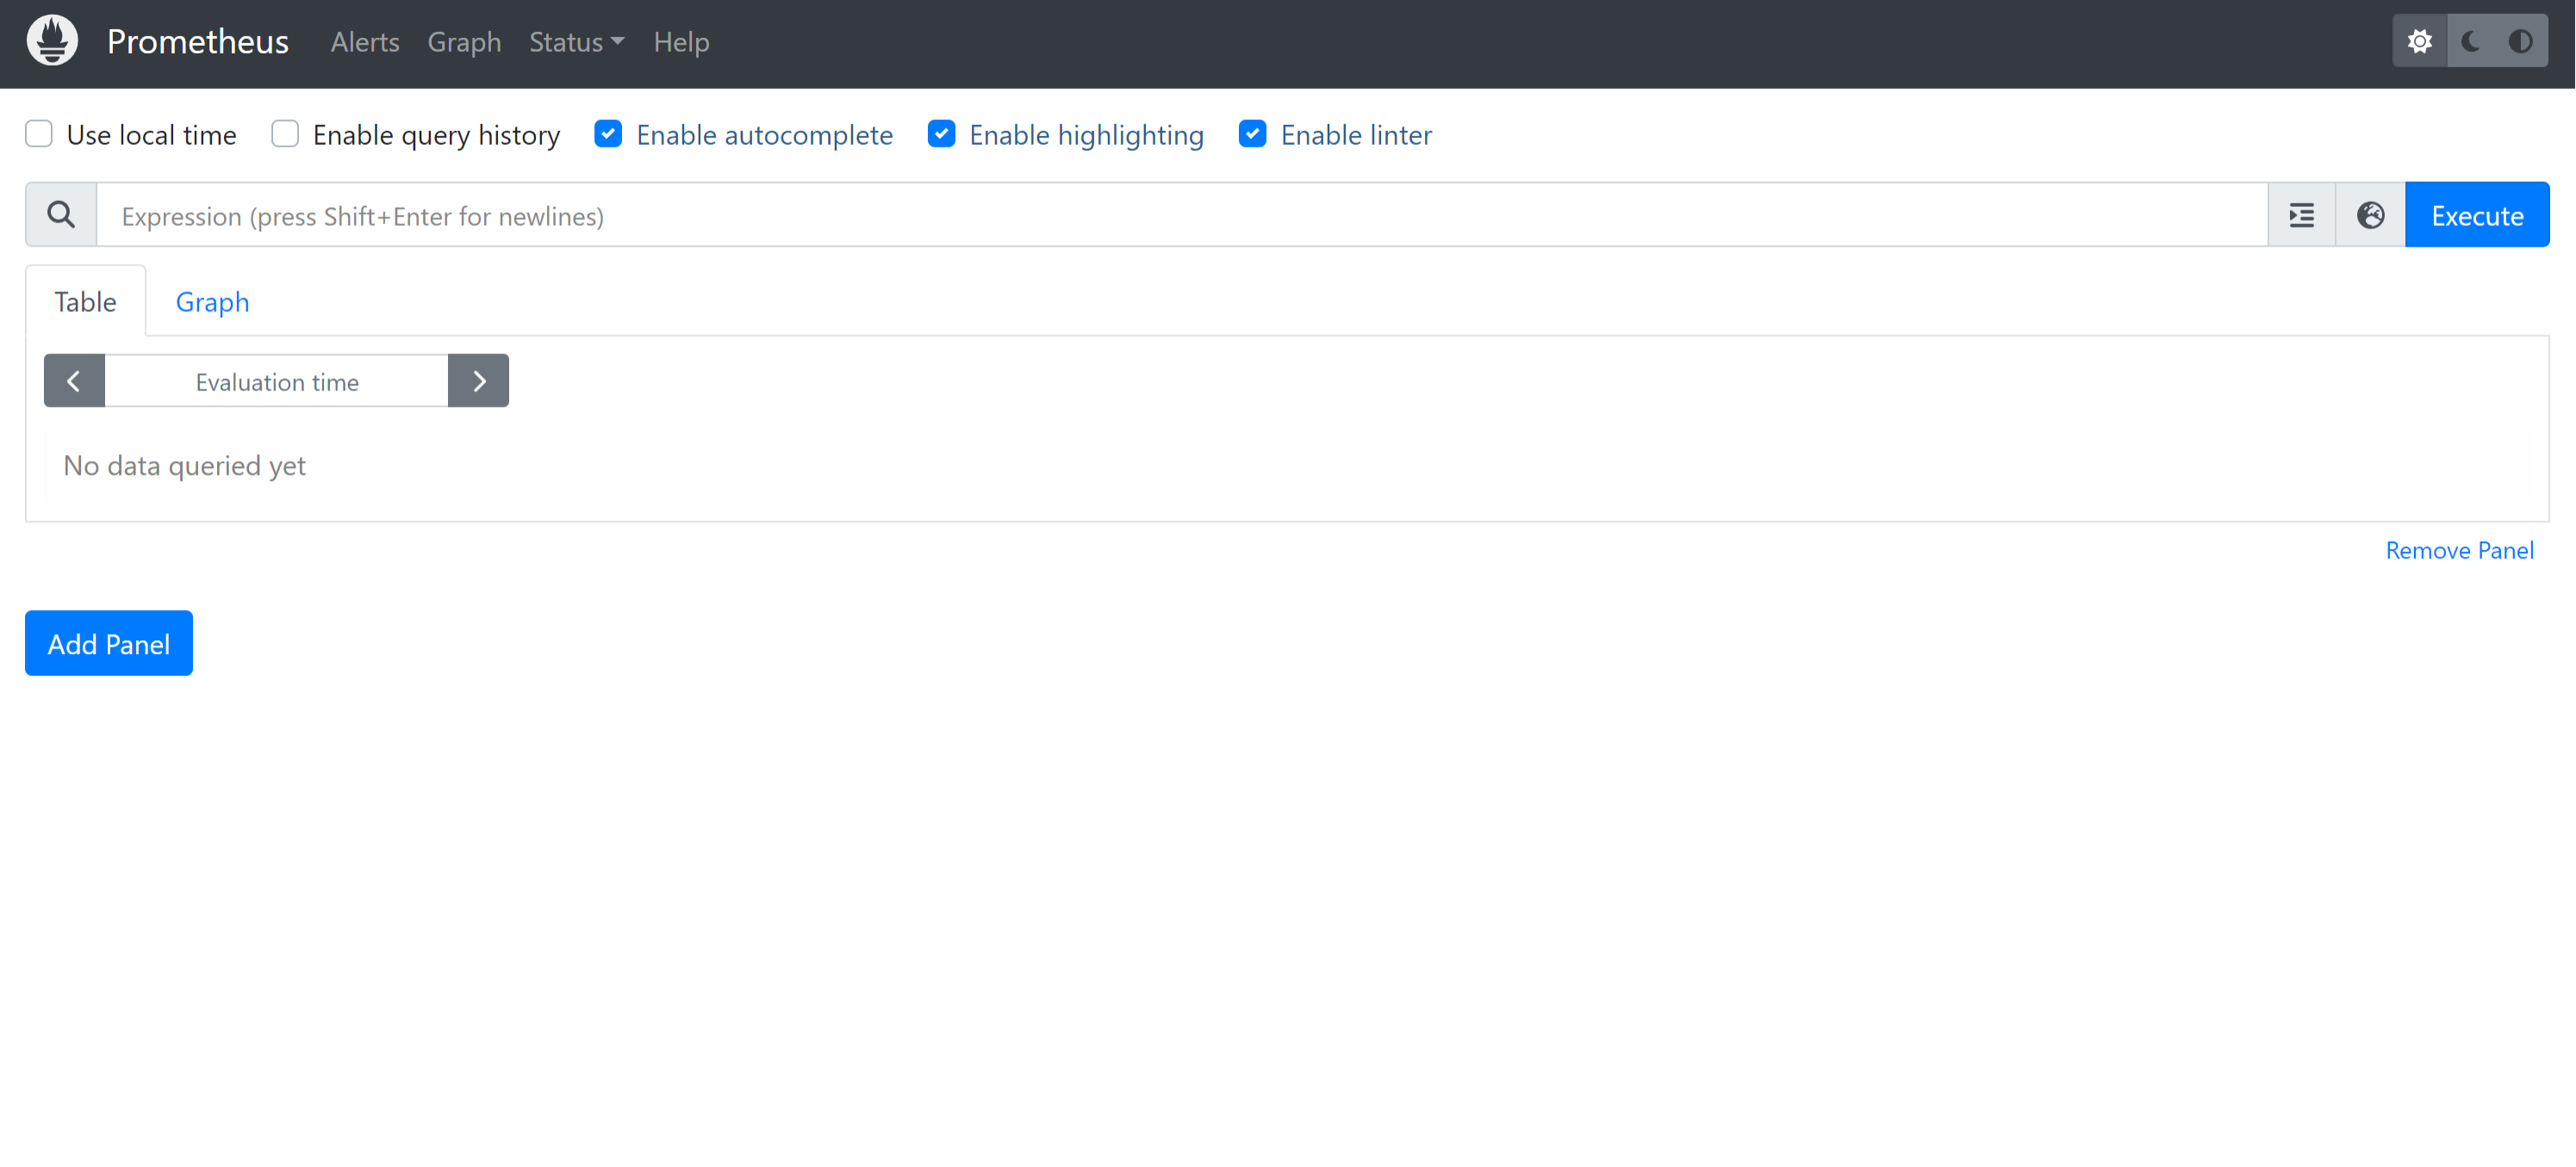
\includegraphics[scale=0.4]{images/hanh/prometheus-dashboard.png}
      \caption{Prometheus dashboard khi vừa mới khởi tạo}
    \end{center}
    \label{}
  \end{figure}

\end{itemize}
\subsubsection{Hiện thực Keda runtime}
\noindent Các ScaledObject của Keda không phải tự nhiên mà có thể vân hành tốt với Kubernetes cluster, mà cần có sư hỗ trợ của keda runtime để có thể vận hành các chức năng cần thiết. May mắn thay, đội ngũ phát triển của Keda đã cung cấp và gói gọn cho chúng ta toàn bộ các cấu hình cần thiết vào trong 1 file cấu hình yaml dài hơn 9700 dòng, mà từ đó ta có thể dễ dàng cài đặt thông qua câu lệnh sau: \lstinline|kubectl apply --server-side -f https://|\lstinline|github.com/kedacore/keda/releases/download/v2.12.1/keda-2.12.1-core.yaml|\\[0.2cm]
Sau khi quá trình cài đặt hoàn tất, ta có thể kiểm tra các dịch vụ đã được cài vào trong cluster thông qua minikube dashboard, namespace \textbf{keda}.
\begin{figure}[H]
  \begin{center}
    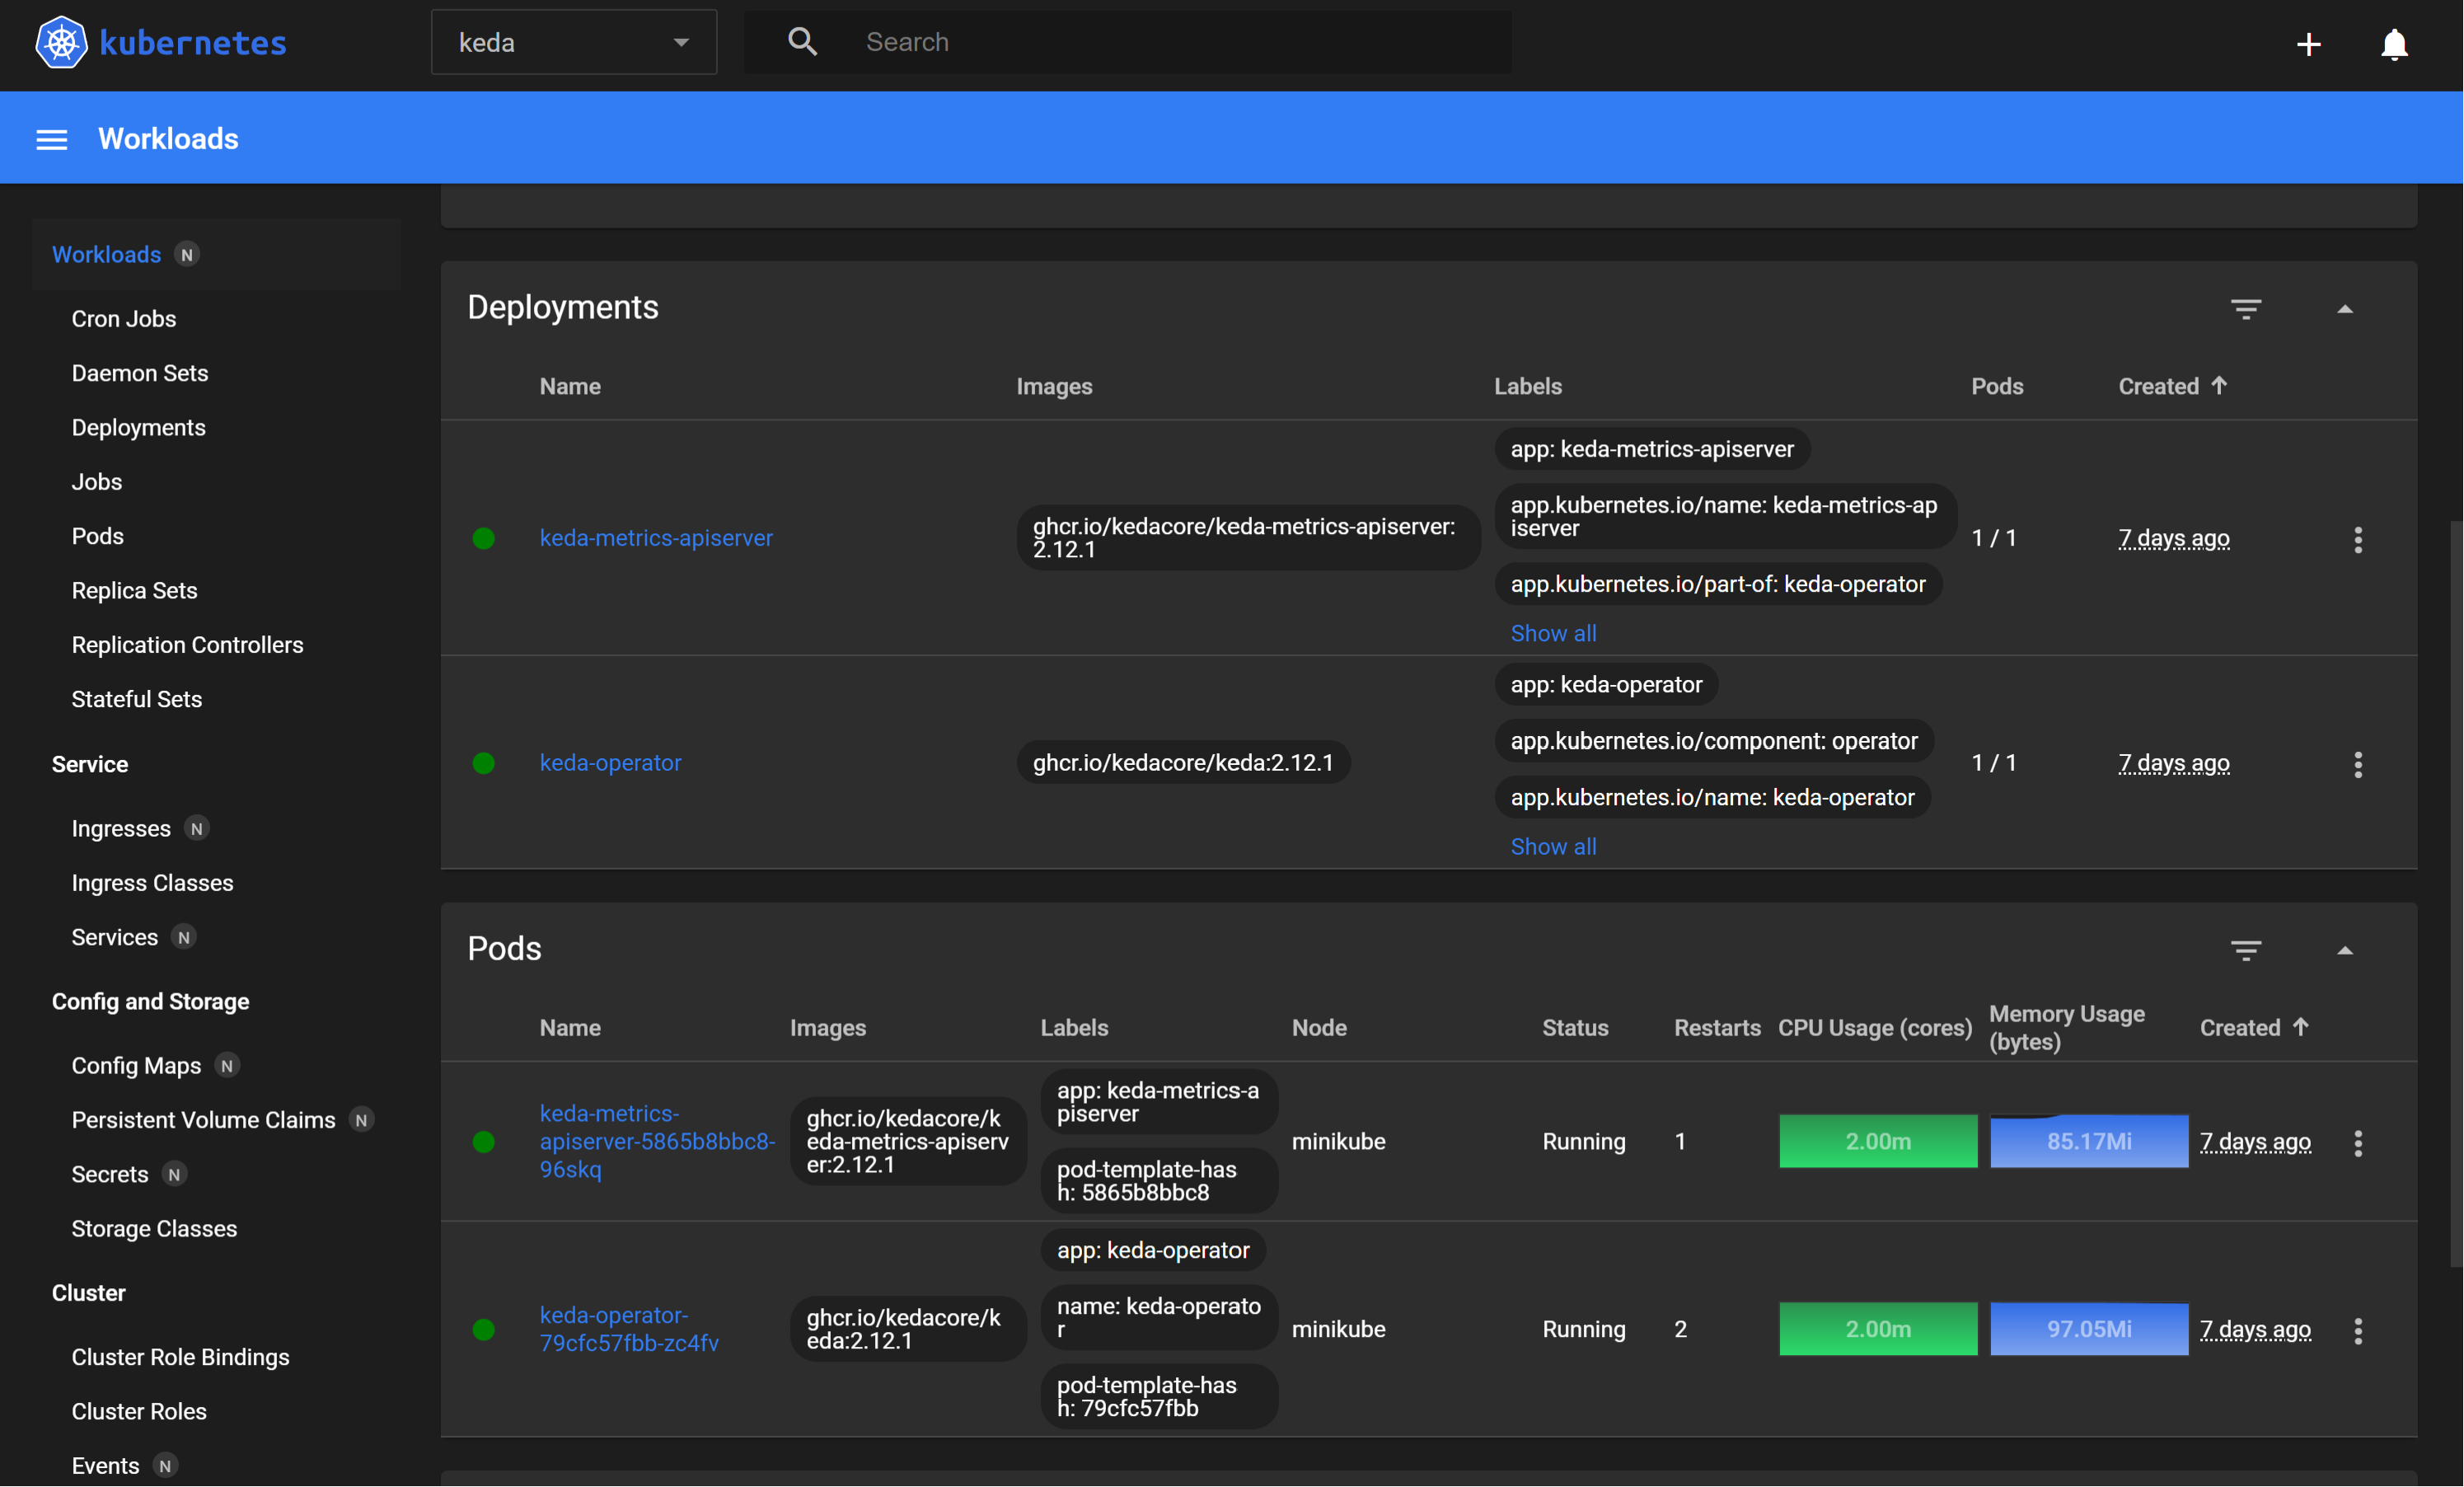
\includegraphics[scale=0.4]{images/hanh/keda-deployment.png}
    \caption{Các deployment và pod phục vụ cho Keda runtime được khởi tạo}
  \end{center}
  \label{}
\end{figure}

\subsubsection{Hiện thực Keda ScaledObject}
\noindent Khi Prometheus server đã sẵn sàng để tiếp nhận thông tin, Keda runtime sẵn sàng cung cấp thông tin đó tới các Keda object thông qua API \lstinline|keda.sh|, thì đó là lúc ta có thể tiến hành cài đặt Keda ScaledObject, nhằm phục vụ cho việc scale theo request của dịch vụ theo cấu hình dưới đây.

\begin{lstlisting}[language=yaml]
apiVersion: keda.sh/v1alpha1
kind: ScaledObject
metadata:
  name: prometheus-scaledobject
  namespace: default
spec:
  scaleTargetRef:
    name: catalog-ms-1-deploy
  pollingInterval: 10  # Optional. Default: 30 seconds
  cooldownPeriod:  15 # Optional. Default: 300 seconds
  minReplicaCount: 1   # Optional. Default: 0
  maxReplicaCount: 10 # Optional. Default: 100
  # fallback:           # Optional. Section to specify fallback options
  #   failureThreshold: 3    # Mandatory if fallback section is included
  #   replicas: 1
  advanced: # Optional. Section to specify advanced options
    horizontalPodAutoscalerConfig: # Optional. Section to specify HPA related options
      behavior: # Optional. Use to modify HPA's scaling behavior
        scaleUp:
          selectPolicy: Max
          stabilizationWindowSeconds: 60
          policies:
            - periodSeconds: 30
              type: Pods
              value: 4
        scaleDown:
          selectPolicy: Min
          stabilizationWindowSeconds: 60
          policies:
            - periodSeconds: 30
              type: Pods
              value: 4
  triggers:
  - type: prometheus
    metadata:
      # Required
      serverAddress: http://prometheus-service.monitoring.svc.cluster.local:8080/
      metricName: access_frequency
      threshold: '1'
      query: sum(rate(node_http_requests_total[1m]))
\end{lstlisting}

\subsection{Kiểm thử}
\subsubsection{Thiết lập}
\noindent Ta sử dụng một tool chuyên dùng để tạo các request gọi tới hệ thống tên là k6, để chạy bài stress test trong các bài kiểm tra lần này. Tool này cho phép ta thiết lập bài kiểm tra bằng javascript thông qua việc \lstinline|export| các biến đã được thống nhất từ trước.\\[0.5cm]
Cấu hình của bài kiểm tra có dạng như sau:
\begin{lstlisting}[language=javascript]
import { check, sleep } from "k6";
import http from "k6/http";

export let options = {
  stages: [
    { duration: "1m", target: 50 },
    { duration: '1m', target: 500 },
    { duration: '2m', target: 1000 },
    { duration: '2m', target: 1200 },
    { duration: "2m", target: 10 },
  ],
};

export default function () {
  let r = http.get(`http://127.0.0.1/catalog`);
  check(r, {
    "status is 200": (r) => r.status === 200,
  });
  sleep(3);
}
\end{lstlisting}
Biến \lstinline|options| có tác dụng xác định bài kiểm tra diễn ra như thế nào. Bài kiếm tra sẽ gồm 5 chặng, mỗi chặng kéo dài lần lượt 1, 1, 2, 2, và 2 phút. Trong thời gian đó, mỗi giây k6 sẽ gửi tương ứng là 50, 500, 1000, 12000 và 10 request về dịch vụ đích, được xác định qua hàm mặc định ở bên dưới. Hàm khởi tạo mặc định này sẽ chứa các thông tin cần thiết về cách kiếm tra, như URL đích của dịch vụ, cũng như các đại lượng cần đo, ở đây là số request được phục vụ thành công, thông qua việc trả về response HTTP 200 OK.
\subsubsection{Kiểm tra khả năng mở rộng của dịch vụ với ScaledObject}
\noindent Trước khi sử dụng một công nghệ nào đó, ta cần xác định xem công nghệ đó có hoạt động như cách ta mong muốn hay không. Ở đây thì ta sẽ kiểm tra xem khi áp dụng ScaledObject thì microservice \textbf{Catalog} có tự scale lên và scale xuống như lý thuyết hay không.\\[0.5cm]
Để theo dõi trạng thái của HPA trong một khoảng thời gian liên tục, ta sử dụng lệnh \lstinline|kubectl get hpa --watch|. Sau đó, ta tiến hành khởi động bài kiểm tra bằng lệnh \lstinline|k6 run api-stress-test.js|.\\[0.5cm]
Sau khi bài kiếm tra kết thúc, ta thu thập được kết quả thông qua terminal như hình dưới.
\begin{figure}[H]
  \begin{center}
    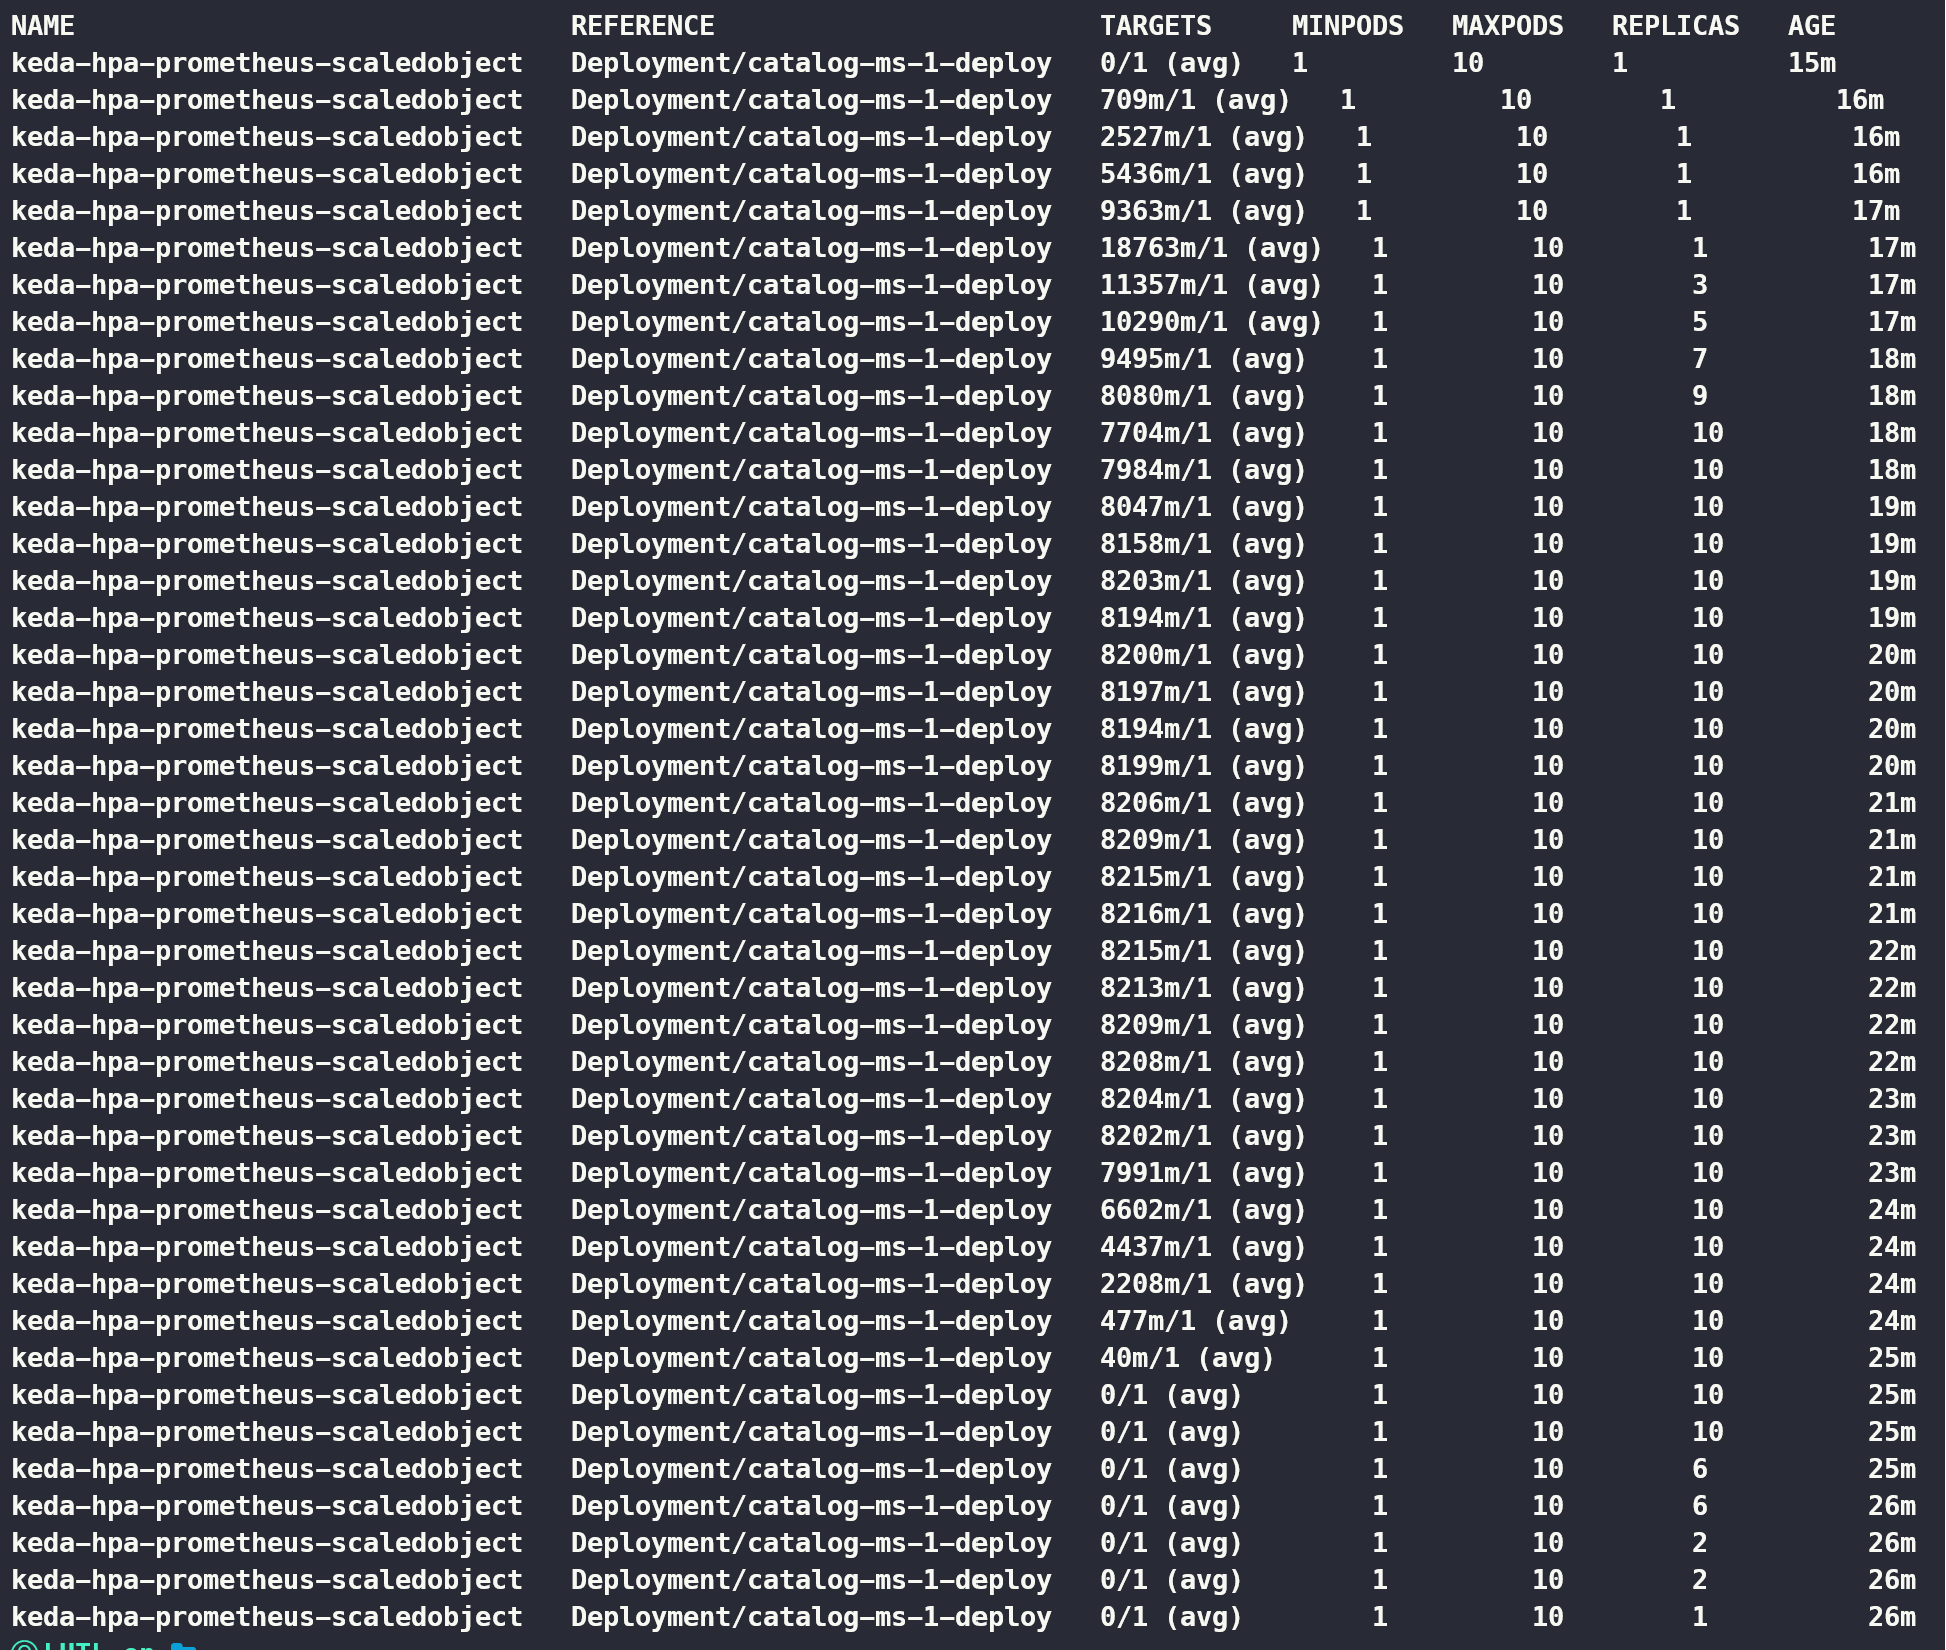
\includegraphics[scale=0.55]{images/hanh/test-with-hpa-pod-scaling.png}
    \caption{Số lượng các pod thay đổi khi chạy bài kiểm tra với k6}
  \end{center}
  \label{}
\end{figure}


Đầu tiên ta thử khi chưa có scale object, kết quả là.
\subsubsection{Kiểm tra tính hiệu quả của việc auto scaling thông qua số request}
Sau đó, ta thử bài test với việc có scale object, kết quả là

Kết luận, k cải thiện dc nhiều do thiếu load balancer.